\documentclass[a4paper]{article}
\usepackage[ngerman]{babel}
\usepackage[T1]{fontenc}
\usepackage[utf8]{inputenc}
\usepackage{pdfpages}
\usepackage{a4wide}
\usepackage{amsmath}
\usepackage{amssymb}
\usepackage{graphics}
\usepackage{mathrsfs}
\usepackage{xspace}
\usepackage{verbatim}
\usepackage{float}
\usepackage{csvsimple}
\usepackage{pgfplotstable} % Generates table from .csv
\usepackage{setspace}
\usepackage{currfile}
\restylefloat{table}
\providecommand{\zB}{z.\,B.\@\xspace}
\providecommand{\Matlab}{\textsc{Matlab}\xspace}
\usepackage[binary-units]{siunitx}
\sisetup{locale = DE}
\sisetup{per-mode = symbol-or-fraction}
\DeclareSIUnit\rounds{U}
\DeclareSIUnit\nmeter{Nm}
\usepackage[breaklinks=true]{hyperref}
\def \Stator {S}
\def \Rotor {R}
\renewcommand{\j}{\jmath}
% Ableitungen
\newcommand{\dd}{\mathop{}\!\mathrm{d}}
\newcommand{\Diff}[2]{\frac{\dd#1}{\dd#2}}
\newcommand{\DiffT}[1]{\Diff{#1}{t}}
\newcommand{\DDiff}[2]{\frac{\dd^2#1}{\dd#2^2}}
\newcommand{\DDiffT}[1]{\DDiff{#1}{t}}
\newcommand{\PartDiff}[2]{\frac{\partial #1}{\partial #2}}
\newcommand{\PartDiffT}[1]{\Diff{#1}{t}}
\newcommand{\PartDDiff}[2]{\frac{\partial^2 #1}{\partial #2^2}}
\newcommand{\PartDDiffT}[1]{\DDiff{#1}{t}}

% Makro für Gleichungen, Abbildungen, Tabellen
\newcommand{\abb}[1]{Abb. \ref{#1}}
\newcommand{\tab}[1]{Tab. \ref{#1}}
\newcommand{\glg}[1]{Glg. \ref{#1}}
\newcommand{\chp}[1]{Kap. \ref{#1}}
\usepackage[european]{circuitikz}
\usepackage{tikz}
\usetikzlibrary{arrows,decorations,intersections, decorations.text,calc}
\usepackage{pgfplots}
\pgfplotsset{compat=1.15}
\usepgfplotslibrary{units}
\pgfplotsset{ticklabel style={/pgf/number format/use comma,/pgf/number format/1000 sep={ }}}
\usetikzlibrary{external}
\tikzexternalize[prefix=tikz/,optimize command away=\includepdf]
\tikzset{external/up to date check=simple}
\tikzset{external/force remake}
\begin{document}

\includepdf{Deckblatt_GSM}
\tableofcontents\newpage
\section{Einleitung}
Bei der verwendeten Maschine, handelt es sich um eine Gleichstrommaschine (GSM) mit Fremderreger- und Reihenschluss-Erregerwicklung. Die Maschine ist als Generator verschalten.\\
Jede der beiden Erregerwicklungen - wenn mit Nennstrom durchflossen - erzeugt daher \SI{50}{\percent} der Nenndurchflutung $\Theta_N$ (siehe auch Nennankerspannung $U_{A,N}$ der GSM). D.h. nur wenn beide Wicklungssysteme Nennstrom führen, stellt sich Nenndurchflutung ein.\\
Die Bemessungsdaten der Gleichstrommaschine können der folgenden Tabelle\;\ref{tab:Nenndaten_GSM} entnommen werden.
\begin{table}[htb]
\begin{center}
\begin{tabular}{ l | l }
\hline
  Bezeichnung & T-T Electric LAK 4132A\\
  Nennankerstrom $I_{A,N}$ & \SI{62}{\ampere}\\
  Nennerregerstrom $I_{E,N}$ & \SI{1.77}{\ampere}\\
  Nenndrehzahl $n_N$ & \SI{2100}{\per \minute}\\
  Nennankerspannung $U_{A,N}$ & \SI{220}{}/\SI{440}{\volt}\\
  Nennerregerspannung $U_{E,N}$ & \SI{220}{\volt}\\
  Wdst. Ankerwicklung $R_A$ & \SI{0.78}{\ohm}\\
  Wdst. Erregerwicklung $R_E$ & \SI{93}{\ohm}\\
  Wdst. Kmpoundwicklung $R_D$ & \SI{0.1}{\ohm}\\
  Kühlung & fremdbelüftet\\
\hline
\end{tabular}
\end{center}
  \caption{Maschinendaten der Gleichstrommaschine (GSM)}
  \label{tab:Nenndaten_GSM}
\end{table}\\
Die Klemmenbezeichnungen für die nachfolgenden Messschaltungen sind in nachstehender Tabelle\;\ref{tab:Klemmenbz_GSM} zusammengefasst.
\begin{table}[htb]
\begin{center}
\begin{tabular}{ l | l }
\hline
  Anker & $A1$-$A2$\\
  Reihenschluss-Erregerwicklung & $D1$-$D2$\\
  Wendepolwicklung & $B1$-$B2$\\
  Fremderregte Erregerwicklung & $F1$-$F2$\\
\hline
\end{tabular}
\end{center}
  \caption{Klemmenbezeichnungen der Gleichstrommaschine (GSM)}
  \label{tab:Klemmenbz_GSM}
\end{table}
\section{Fremderregter Gleichstromgenerator}
Beim fremderregten Gleichstromgenerator wird die Hauptfelderregung $\Theta_E$ über einen separaten Erregerkreis (Erregerwicklung $F1$-$F2$) eingestellt und kann daher unabhängig vom Laststrom $I_A$ und der Drehzahl $n$ gewählt werden.\\
\subsection{Leerlaufkennlinien}
\begin{figure} [htb]
    \centering
    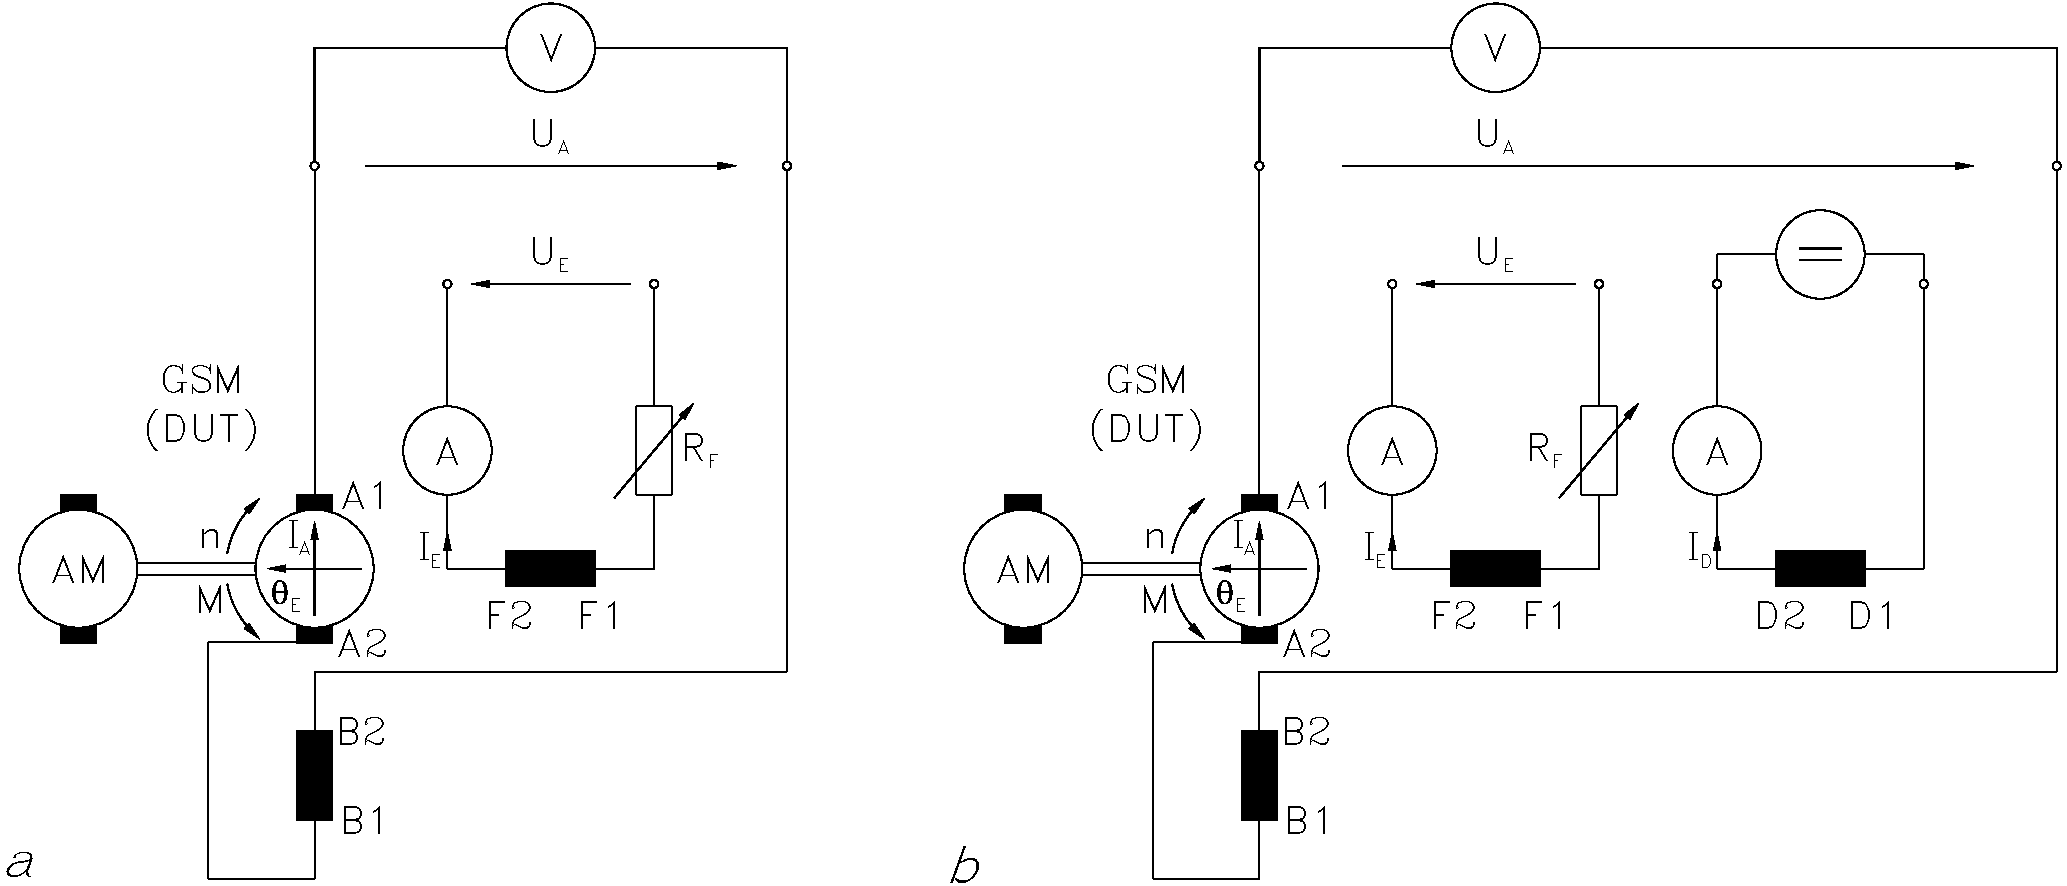
\includegraphics[width=1\textwidth, angle=0]{\currfiledir images/Leerlaufkennlinie_fremd_und_RS}
    \caption{Messschaltungen zur Ermittlung der Leerlaufkennlinie: (a) fremderregter Gleichstromgenerator (GSM), (b) fremderregter Gleichstromgenerator mit fremdbestromter Reihenschlusswicklung ($D1$-$D2$).}
    \label{abb:fremd_LL_Messschaltung}
\end{figure}
\noindent Die Leerlaufkennlinie stellt die innere Spannung in Abhängigkeit der Durchflutung bzw. des Erregerstromes bei konstanter Drehzahl dar.\\
Für deren Bestimmung wird daher eine konstante Drehzahl ($n=n_N$) über die Antriebsmaschine ($AM$) eingeprägt und (bei offenen Klemmen, $I_A = 0$) die innere Spannung $U_A=U_i$ gemessen.\\
Da die Maschine zwei Erregerwicklungen besitzt, wurden zwei Messungen durchgeführt.\\
Bei der ersten Messung wurde die Maschine nur fremderregt betrieben, d.h. die Erregerwicklung $F1$-$F2$ wurde über die Hausbatterie des Labors mit Nennspannung $U_E=U_{E,N}$ versorgt und über einen Vorwiderstand $R_F$ der Erregerstrom $I_E$ variiert. Im zweiten Durchgang wurde die Reihenschlusswicklung ($D1$-$D2$) mit konstanten \SI{40}{\ampere} bestromt und der Strom durch die fremderregte Erregerwicklung wieder variiert. D.h. die Reihenschlusswicklung liefert ihrerseits einen konstanten Erregerbeitrag von $\approx\SI{30}{\percent}$ der Nennerregung $\Theta_{E,N}$.\\
Damit ergeben sich eine Leerlaufkennlinie für die (rein) fremderregte GSM (\SI{0}{}-\SI{50}{\percent} Flussniveau, siehe Abb.\;\ref{abb:fremd_LL_BL_Innen}) und für die Kombination der beiden Erregerwicklungen (\SI{0}{}-\SI{80}{\percent} Flussniveau, siehe Abb.\;\ref{abb:fremd_reihen_LL}).


\subsection{Belastungskennlinie}
\begin{figure} [htb]
    \centering
    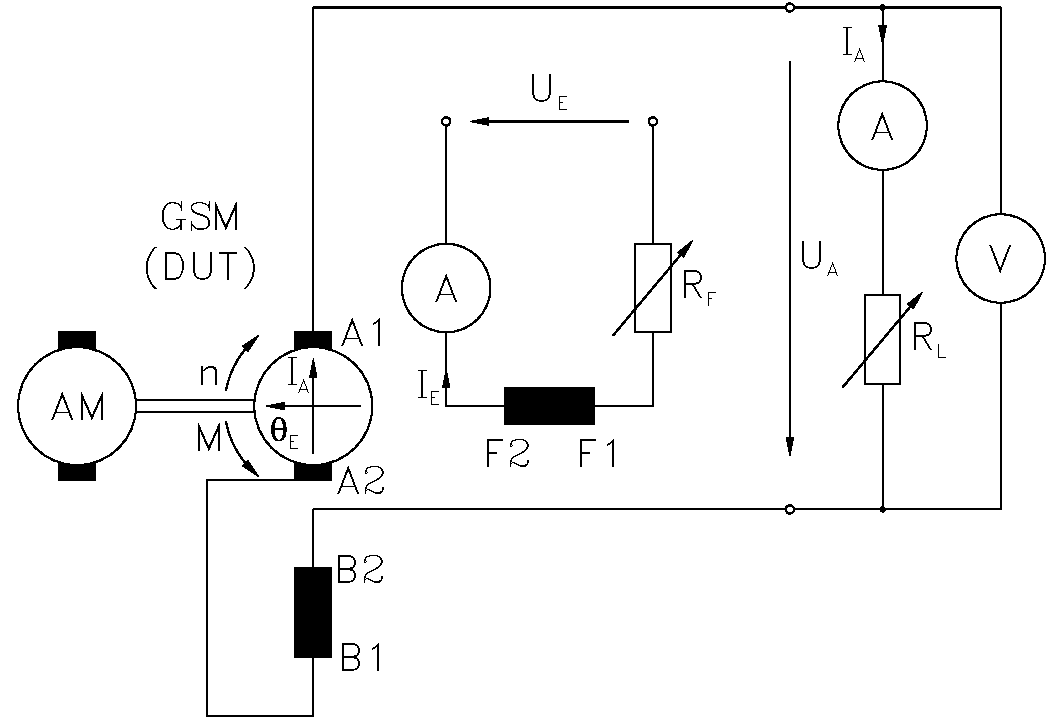
\includegraphics[width=0.55\textwidth, angle=0]{\currfiledir images/Belastungskennlinie_fremderregt}
    \caption{Messschaltung zur Ermittlung der Belastungskennlinie (äußeren Kennlinie und der Regulierkennlinie) des fremderregten Gleichstromgenerators (GSM).}
    \label{abb:fremd_BKL_Messschaltung}
\end{figure}
Nun wurde die Schaltung über einen Leistungswiderstand $R_L$ belastet. Die Drehzahl bleibt dabei unverändert bei $n=n_N$, während Nennerregung $I_E=\SI{1.75}{\ampere}$ gewählt wurde. Der Belastungswiderstand wurde so eingestellt, dass der Ankerstrom bei \SI{50}{\ampere} und die Klemmenspannung bei \SI{200}{\volt} zu liegen kommen. Nun wurde der Erregerstrom stufenweise reduziert und der Ankerstrom über den Belastungswiderstand konstant gehalten. Die resultierende Kennlinie ist in Abbildung \ref{tab:Fremderregt_Belastung} zu sehen. Diese liegt aufgrund der Flussminderung durch den Ankerstrom und den Spannungsabfall am Ankerwiderstand $R_A$ unterhalb der Leerlaufkennlinie.
\subsection{Äußere Kennlinie}
Bei der Äußeren Kennlinie wird die Ankerspannung in Abhängigkeit des Ankerstroms bei konstanter Drehzahl $n=n_N$ aufgenommen. Zu Beginn wird der Erregerstrom $I_E$ so gewählt, dass sich eine Klemmenspannung von \SI{200}{\volt} und ein Ankerstrom von \SI{50}{\ampere} einstellt. Danach wurde die Klemmenspannung gemssen während der Belastungswiderstand $R_L$ schrittweise erhöht wurde, wodurch der Ankerstrom sinkt. Die Gleichung
\begin{equation*}
    U_A=U_i - R_A I_A
\end{equation*}
beschreibt das vorliegende Verhalten in Abbildung \ref{abb:fremd_aussen_regulier} sehr gut. Die GSM verhält sich also wie eine ideale Spannungsquelle mit Innenwiderstand. Für höhere Ströme bzw. eine höhere Erregung wird das lineare Verhalten durch die enstehende Ankerrückwirkung durch die Sättigung des Eisens verzerrt.
\subsection{Innere Kennlinie}
Die Innere Kennlinie lässt sich aus der Belastungskennlinie berechnen. Ein Blick auf die Messschaltung \ref{abb:fremd_BKL_Messschaltung} liefert folgende Gleichung:
\begin{equation*}
    U_i=U_A + R_A I_A
\end{equation*}
Der Wert für den Ankerwiderstand $R_A$ kann den Maschinendaten entnommen werden und entspricht \SI{0.78}{\ohm}. Die so entstandene Kennlinie ist in Abbildung \ref{abb:fremd_LL_BL_Innen} dargestellt.
\subsection{Regulierkennlinie}
Bei der Regulierkennlinie wird der Erregerstrom $I_E$ als Funktion des Ankerstroms $I_A$ dargestellt. Dabei wird die Ankerspannung konstant auf \SI{200}{\volt} gehalten und die Drehzahl wieder auf $n=n_N$ eingestellt.\\
Der Belastungsstrom wurd durch den Lastwiderstand $R_L$ variiert und im Anschluss wird der Erregerstrom über den Vorwiderstand manuell geregelt, sodass sich wieder eine Klemmenspannung von \SI{200}{\volt} ergibt. In Abbildung \ref{abb:fremd_aussen_regulier} ist der Verlauf zu sehen. Die Beziehung zwischen dem Felderregerstrom $I_E$ und dem Ankerstrom $I_A$ ist nahezu linear. Das liegt daran, dass bei steigender Belastung die induzierte Spannung und somit der magnetische Fluss steigen müssen, um die Spannung $U_A$ konstant halten zu können. Bei einer höheren Belastung als Nennstrom $I_{A,N}$ steigt der benötigte Erregerstrom $I_E$ überproportional an, da nun das Eisen zu sättigen beginnt. Die Folge ist eine Kennlinie die bis ungefähr $I_A = I_{A,N}$ linear verläuft.
\input{\currfiledir Fremd_und_Reihen_LL}
\input{\currfiledir Fremderregt_LL_BL_Innen}
\input{\currfiledir Fremderregt_Aussen_Regulier}
%\input{\currfiledir schaltung}
\section{Nebenschlussgenerator}
Bei diesem Generatortyp liefert der Generator selbst den Erregerstrom zum Feldaufbau, da die Erregerwicklung parallel geschaltet wird (siehe Abbildung \ref{abb:neben_BKL_Messschaltung}). Zum Anlaufen ohne externe Spannung wird die Remanenz ausgenutzt, dabei ist bei der Verschaltung der Wicklung auf eine positive Rückkopplung zu achten, da sonst der vom Erregerstrom $I_E$ erregt Fluss $\Phi$ die zum Remanenzfluss $\Phi_R$ entgegengesetzte Polarität aufweist, ihn somit schwächt, sodass der Selbsterregungsprozess nicht zustande kommt. Dies kann sogar zur Entmagnetisierung der Maschine führen, worauf für ein erneutes Anfahren eine fremde Erregung benötigt wird.\\

\subsection{Äußere Kennlinie}
\begin{figure} [htb]
    \centering
    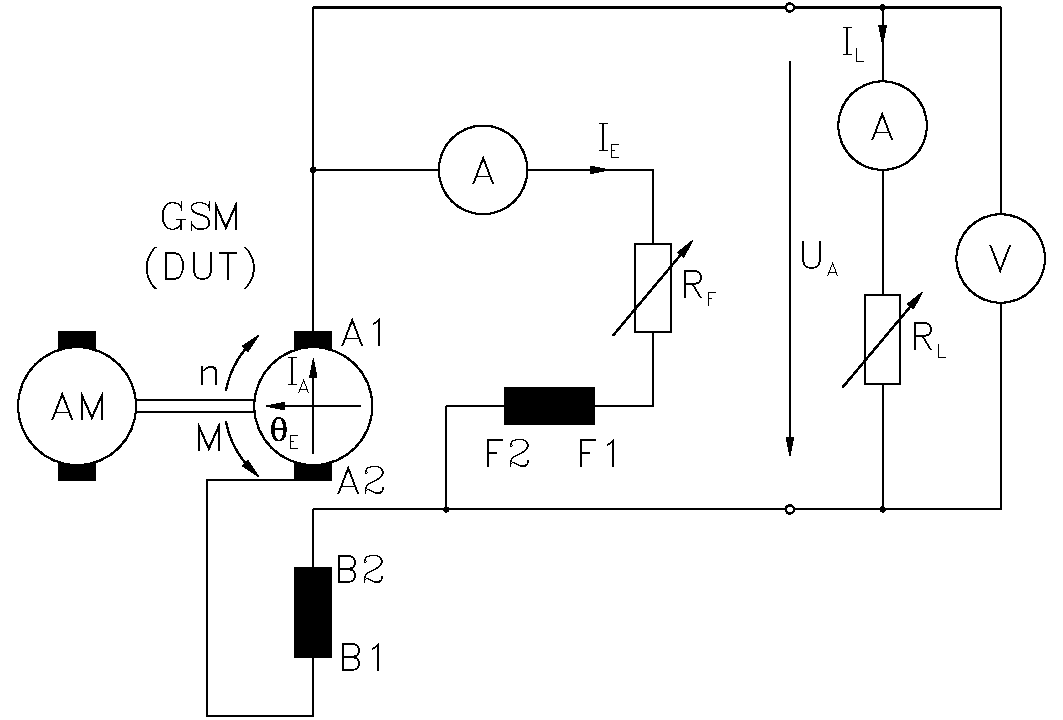
\includegraphics[width=0.55\textwidth, angle=0]{\currfiledir images/Belastungskennlinie_nebenerregt}
    \caption{Messschaltung zur Ermittlung der äußeren Kennlinie des Nebenschluss\-gleich\-strom\-generators (GSM).}
    \label{abb:neben_BKL_Messschaltung}
\end{figure}
\noindent Bei der Äußeren Kennlinie wird der Verlauf der Ausgangsspannung $U_A$ in Abhängigkeit der Belastung, d.h. des Ausgangsstromes $I_L$ ermittelt.\\
Dazu wird die Gleichstrommaschine wieder über die Antriebsmaschinen auf Nenndrehzahl $n=n_N$ beschleunigt und gehalten.\\
Der Startpunkt der Messung wird über die Widerstände $R_L$ und $R_F$ so gewählt, dass sich für einen Felderregerstrom $I_E=\SI{1.65}{\ampere}$ eine Ausgangsspannung $U_A=\SI{200}{\volt}$ einstellt. Anschließend wird die Belastung reduziert, d.h. der Widerstand $R_L$ erhöht, bis sich der Erregerstrom auf $\approx1.2\,I_{E,N}$ erhöht. Um den Einfluss der Hysterese zu minimieren, wird bei der folgenden Kennlinienaufnahme, die Belastung stets erhöht, d.h. der Widerstand $R_L$ kontinuierlich verringert.\\
Die daraus erhaltene äußere Kennlinie des Nebenschlussgenerators ist in Abbildung\;\ref{abb:nebenschluss_aussen} ersichtlich.\\
Im Vergleich zur äußeren Kennlinie des fremderregten Gleichstromgenerators (siehe Abb.\;\ref{abb:fremd_aussen_regulier}, Ankerspannung $U_A$), ist vor allem die stärkere Abhängigkeit der Ausgangsspannung $U_A$ vom Ausgangsstrom $I_A$ offensichtlich.\\
Bei Belastung sinkt durch den ohmschen Spannungsabfall am Ankerwiderstand $R_A$ die Ankerspannung. Dadurch sinkt auch die an der Nebenschlusswicklung anliegende Spannung und damit der von ihr getriebene Erregerstrom $I_E$ und somit der Fluss, sodass die Ankerspannung stärker sinkt als beim fremderregten Generator (konstante Erregerspannung). D.h. die Ausgangsspannung des Nebenschlussgenerators sinkt überproportional mit steigendem Ausgangsstrom, d.h. stärker als der ohmsche Spannungsabfall am Ankerwiderstand (vgl. Abb.\;\ref{abb:fremd_aussen_regulier}) es vermuten lässt.\\
Schließlich tritt aufgrund der fehlenden Kompensationswicklung bei sehr hohen Ankerströmen, die Ankerrückwirkung in Form einer globalen Feldschwächung in Erscheinung. Durch das geschwächte Hauptfeld wird weniger Spannung in die Maschine induziert, was eine weitere Reduktion der Ankerspannung nach sich zieht.\\
Wird die Maschine noch stärker belastet, so wird ein Punkt der Kennlinie erreicht, ab dem durch eine weitere Reduktion des Lastwiderstandes keine Erhöhung des Ausgangsstromes mehr erreicht werden kann. Der Erregerstrom und damit das Feld und schließlich die Ankerspannung, nehmen soweit ab, dass auch der Ausgangsstrom wieder zu sinken beginnt.\\
Der Kurzschlusspunkt des Generators stellt sich bei kurzgeschlossenem Ausgang ein (Felderregerstrom $I_E=0$), wobei aufgrund des Remanenzflusses $\Phi_R$ in der Maschine zumindest die Remanenzspannung $U_R$ induziert wird. Der Ausgangsstrom $I_L$ aus dem Generator wird durch den Ankerwiderstand begrenzt.\\
Der Kurzschlusspunkt konnte aufgrund des Mindestwertes des verwendeten Lastwiderstandes nicht erreicht werden.\\
Aufgrund der Erwärmung der Maschine während der Messung, ergibt sich der nicht-ideale Verlauf der Kurvenform (Dellen).
\input{\currfiledir Nebenschluss}
%\input{\currfiledir schaltung}
\section{Reihenschlussgenerator}
Bei diesem Generatortyp wird die Erregerwicklung in Serie mit der Ankerwicklung geschaltet. Da nun der Ankerstrom (=Erregerstrom) durch die Erregerwicklung ($D1$-$D2$) fließt, muss die Wicklung für deutlich höhere Ströme ausgelegt sein (wenige Windungen mit entsprechend größerem Querschnitt als bei der Fremd- oder Nebenschlusswicklung). Auch hier ist wieder auf den korrekten Stromfluss durch die Wicklung bei der Verschaltung zu achten, da die Maschine ansonsten ihren vorhandenen Remanenzfuss $\Phi_R$ durch die . Die Schaltung für den Reihenschlussgenerator ist in Abbildung \ref{abb:reihen_BKL_Messschaltung} dargestellt. 
\subsection{Bremsversuch}
\begin{figure} [htb]
    \centering
    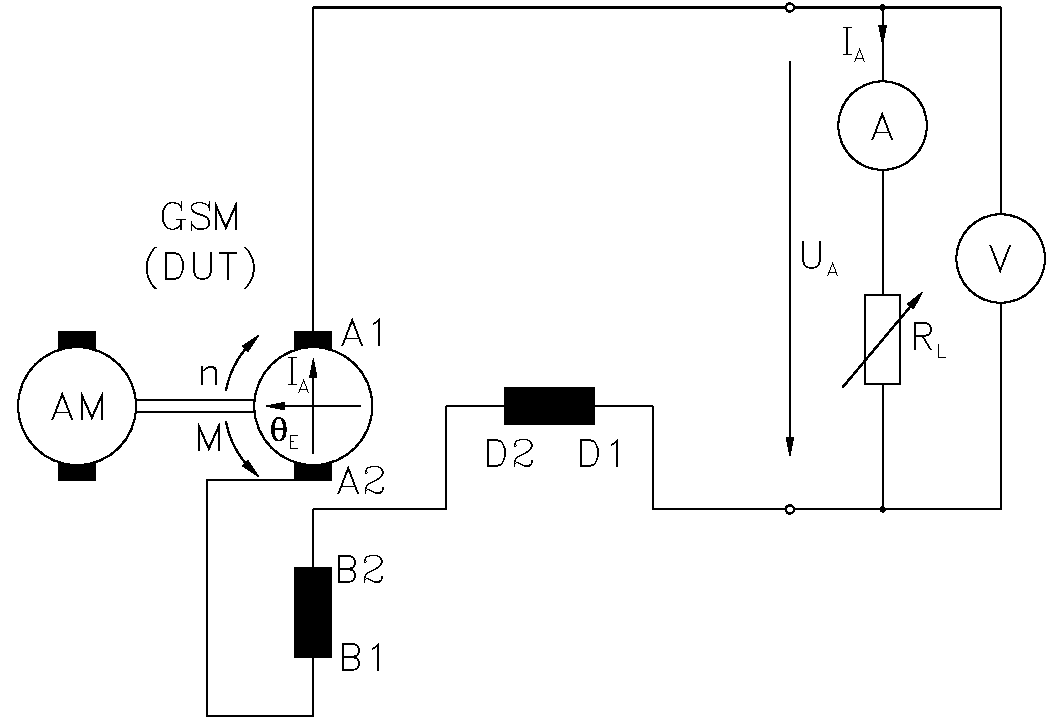
\includegraphics[width=0.55\textwidth, angle=0]{\currfiledir images/Bremskennlinie_reihenerregt}
    \caption{Messschaltung zur Durchführung eines Bremsversuchs des Reihen\-schluss\-gleich\-strom\-generators (GSM).}
    \label{abb:reihen_BKL_Messschaltung}
\end{figure}
Die erste Messung ist die äußere Kennlinie der Maschine, also der Verlauf der Ankerspannung in Abhängigkeit des Ankerstroms. Die Drehzahl wurde auf die negative Nenndrehzahl  ($n=n_N$) eingestellt. Die Belastung wurde über den Widerstand $R_L$ festgelegt, wodurch der Ankerstrom variiert wurde. Die so entstandene Kennlinie ist in Abbildung \ref{abb:reihenschluss_aussen} zu sehen.
\subsection{Innere Kennlinie}
Um die innere Kennlinie der Reihenschlussmaschine zu berechnen, wird die Äußere Kennlinie mit der folgenden Formel umgerechnet.
\begin{equation*}
    U_i=U_A + (R_A+R_D) I_A
\end{equation*}
Die Widerstandswerte können dem Maschinendatenblatt entnommen werden und entsprechen $R_A = \SI{0.78}{\ohm}$ und $R_D = \SI{0.1}{\ohm}$. Der Verlauf der Kennlinie ist ebenfalls in Abbildung \ref{abb:reihenschluss_aussen} dargestellt.
\input{\currfiledir Reihenschluss}
%\input{\currfiledir schaltung}
\section{Verbundgenerator}
Die letzte zu untersuchende Maschine ist ein Verbundgleichstromgenerator. Dieser vereint in unserem Fall einen fremderregten Generator mit einem Reihenschlussgenerator. Dazu wird die Fremderregerwicklung sowie die Reihenschlusswicklung wie in Abbildung \ref{abb:verbund_BKL_Messschaltung} verschaltet. Dadurch wird das Hauptfeld in Abhängigkeit von $R_S$ proportional zum Ankerstrom erhöht, wodurch zum Beispiel die Ankerrückwirkung reduziert werden kann. Die Erregung ist nun über zwei Widerstände regelbar - einerseits über den Fremderregerwiderstand, andererseits durch Variation des zur Hilfsreihenschlusswicklung parallel geschalteten Widerstands $R_S$. Wird dieser erhöht, fließt mehr Ankerstrom durch die Wicklung, was eine erhöhte Erregung zur Folge hat. Bei Verringerung des Widerstandes zapft dieser in der Parallelschaltung mehr Strom ab, wodurch die Erregerdurchflutung sinkt. 

\begin{figure} [htb]
    \centering
    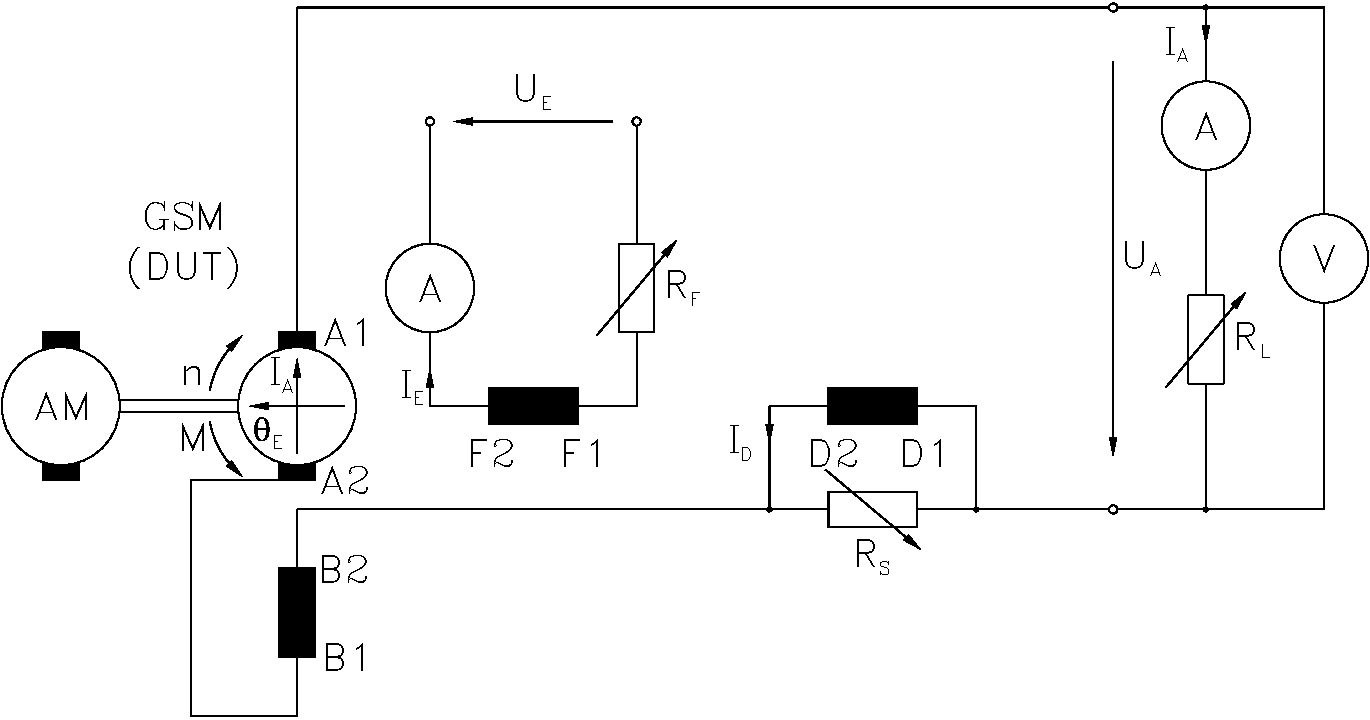
\includegraphics[width=0.75\textwidth, angle=0]{\currfiledir images/Belastungskennlinie_verbunderregt}
    \caption{Messschaltung zur Ermittlung der äußeren Kennlinie des Verbund\-gleich\-strom\-generators (GSM) - Reihenschlusswicklung hier dargestellt für Kompoundierung (für Gegenkompoundierung müssen die Anschlüsse der Reihenwicklung $D1$ und $D2$ vertauscht werden).}
    \label{abb:verbund_BKL_Messschaltung}
\end{figure}

\subsection{Äußere Kennlinie}

Bei der äußeren Kennlinie wurden drei verschiedene Konfigurationen - überkompoundiert, kompoundiert und gegenkompoundiert - aufgenommen, auf die in Folge näher eingegangen wird. Dabei wurde jeweils der Widerstand $R_S$ fix vorgegeben und der Belastungswiderstand $R_L$ bei Nenndrehzahl und Nenn-Fremderregung ($I_{F,N}= \SI{1.75}{\ampere}$) variiert. Abbildung \ref{abb:verbund_kennlinien} zeigt die gemessenen äußeren Kennlinien als durchgezogene Linien für jeden dieser Fälle.

\subsubsection{Überkompoundiert}

Bei der Überkompoundierung ist es nicht nur das Ziel, die Ankerrückwirkung zu kompensieren, sondern darüber hinaus die Erregung proportional mit dem Ankerstrom zu verstärken und damit im Generatorbetrieb eine erhöhte Ankerspannung zu erhalten. Die abnehmende Steigung der Kennlinie bei zunehmendem Strom rührt aus der maximal verfügbaren Leistung der Antriebsmaschine. 

\subsubsection{Kompoundiert}

Bei der reinen Kompoundierung wird versucht, das schwächende Feld der Ankerrückwirkung durch die Hilfsreihenschlusswicklung exakt zu kompensieren und somit eine belastungsunabhängige Charakteristik zu erzielen. Es ist zu erkennen, dass dies nicht gänzlich gelingt - für ein noch besseres Ergebnis wäre der Parallelwiderstand $R_S$ weiter zu senken. 

\subsubsection{Gegenkompoundiert}

Vertauscht man die Klemmen der Hilfsreihenschlusswicklung, so wird der gegenteilige Effekt erzielt: Das von ihr erzeugte Feld wirkt zusammen mit der Ankerrückwirkung der Erregung entgegen und bewirkt damit ein starkes Einbrechen der Ankerspannung mit steigendem Strom.

\subsection{Innere Kennlinien}

Für die inneren Kennlinien der verschiedenen Betriebszustände werden die äußeren herangezogen und entsprechend 

\begin{equation}
U_i=U_A+I_A R_A
\end{equation}

\noindent umgerechnet. Der vergleichsweise ohnehin niedrige Widerstand der Hilfsreihenschlusswicklung $R_D$ wird durch die Paralllelschaltung mit $R_S$ weiter verringert, weshalb diese vernachlässigt und nur der Ankerkreiswiderstand herangezogen wird. Die Ergebnisse sind ebenfalls in Abbildung \ref{abb:verbund_kennlinien} grafisch dargestellt, im Gegensatz zu den äußeren Kennlinien jedoch strichliert.

\input{\currfiledir Verbund}
%\input{\currfiledir schaltung}
\section{Anhang}
Lorem ipsum dolor sit amet, consectetur adipiscing elit. Mauris fringilla suscipit faucibus. Duis tincidunt, augue et dapibus lacinia, tortor mi viverra sapien, non ullamcorper odio risus a mauris. Maecenas at libero et mauris scelerisque sollicitudin quis sed orci. Donec congue ante felis, rutrum commodo lorem auctor quis. In consequat luctus turpis et vulputate. In sit amet rhoncus risus, porta imperdiet ex. Morbi neque lacus, consectetur quis dictum quis, pulvinar ac urna. Aliquam in dolor ut erat facilisis fringilla. Sed molestie commodo est.

Mauris sit amet eros sem. Donec quam massa, luctus ut nunc at, dignissim ornare augue. Aenean sagittis consequat nulla quis facilisis. Duis ultricies laoreet dui, ut condimentum arcu sodales sit amet. Nullam efficitur tellus vel faucibus scelerisque. Duis varius felis vitae eros maximus vestibulum. In porttitor pellentesque tellus, vel placerat orci. Phasellus consequat libero purus, sit amet semper ipsum fermentum non. Quisque rutrum sapien lectus, at faucibus eros egestas eget. Nulla id nisi tortor. Morbi porttitor interdum porta.

Morbi porta dolor metus, eget hendrerit justo ullamcorper ut. Vivamus commodo, arcu quis finibus eleifend, odio sem dignissim orci, nec pellentesque sapien metus at tortor. Sed dictum lectus suscipit imperdiet ultrices. Proin tellus neque, ornare sed mattis vel, faucibus at turpis. Lorem ipsum dolor sit amet, consectetur adipiscing elit. Morbi sit amet condimentum risus, nec lobortis sem. Donec molestie vel dui in egestas. Quisque tellus nisl, suscipit at viverra eget, aliquam eu est. Nam cursus nunc ultrices, pulvinar lorem vel, ullamcorper ante. Nunc sed dolor nec tellus commodo vehicula.

Phasellus id arcu sed enim sodales fringilla at nec metus. Mauris vel nibh et nibh bibendum gravida ut at metus. Sed bibendum, dui nec congue sodales, quam urna gravida lorem, sed vestibulum velit mi nec lorem. Quisque placerat congue ullamcorper. Vestibulum sollicitudin enim at risus gravida suscipit. Maecenas blandit consectetur enim, sed maximus diam dignissim at. Nam venenatis erat eleifend velit posuere accumsan. Nunc bibendum felis ac elit posuere venenatis. Suspendisse aliquet quam magna. Aenean quis ante posuere, interdum quam ut, accumsan ex.

Fusce molestie lacinia maximus. Suspendisse eget ex nec orci ullamcorper euismod auctor sed dui. Vivamus iaculis egestas tellus non consectetur. Sed dapibus vitae felis in gravida. Donec sapien sem, euismod et tincidunt egestas, bibendum eget odio. Nulla sed sapien efficitur, mattis metus ac, aliquam leo. Integer consequat bibendum turpis, at rhoncus purus sodales eget. Aenean quis accumsan velit.
\end{document}
